\section{Einkauf}
\autorbeginn{Marcel}
\label{sec:ui-einkauf}

Zur Produktion der Raumschiffe werden diverse Bauteile benötigt. Hierzu steht der Bildschirm „Einkauf“ dem Spieler zur Verfügung.
 
Im oberen Teil des Bildschirms befinden sich drei Container, die jeweils zu den Triebwerken, Rumpfbauteilen und Hitzeschildern alle notwendigen Daten enthalten. Ein solcher Container soll anhand des Containers „Triebwerke“ näher erläutert werden. 
 
Der Container Triebwerk enthält ein Bild des zum Einkauf angebotenen Triebwerks. Innerhalb des Bildes befindet sich ein Hilfebutton, der in Form eines Fragezeichens dargestellt wird. Über diesen Button erscheint ein PopUp-Fenster, das dem Spieler umfassende Informationen zu dem Triebwerk und zur benötigten Anzahl der Triebwerke pro Raumschiff liefert. Rechts neben diesem Bild kann der Spieler die Anzahl gewünschte Anzahl einzukaufender Triebwerke angeben.
 
Neben dem aktuellen Marktpreis des  Triebwerks, der sich unterhalb der gewünschten Stückzahl befindet, kann der Spieler über einen weiteren Button die Preisentwicklung von Triebwerken auf dem Einkaufsmarkt anschauen. Bei Betätigung des Buttons, öffnet sich ein PopUp, das ein Liniendiagramm der aktuellen Preisentwicklung enthält. Im unteren Teil des Containers Triebwerk wird mittig der Gesamtpreis der Triebwerke bei gewünschter Anzahl angezeigt. \ref{img:ui-triebwerk}  zeigt den Container Triebwerk.

% Bitte verschiedene Captions wählen
\begin{figure}[htb]
  \centering
  \fbox{
    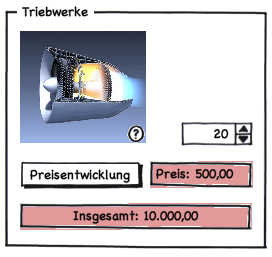
\includegraphics[width=0.45\textwidth]{40_UI/50_Einkauf/Container_Triebwerk.png}
  }
  \caption{Einkauf}
  \label{img:ui-triebwerk}
\end{figure}
 
In ähnlichen Containern werden auf dem Einkaufsbildschirm auch die Sonderbauteile des jeweiligen Raumschiffes angezeigt. In diesen hat der Spieler jedoch nur die Option, die gewünschte Anzahl der Bauteile anzugeben, sowie den Bauteilpreis einzusehen.
 
Der gesamte Einkaufspreis wird in roter Schrift rechts neben den Sonderbauteilen dargestellt. Darüber befindet sich ebenso das aktuelle Bankguthaben, sodass der Spieler mit Hinblick auf die aktuelle Finanzsituation des Unternehmens handelt. Hat der Spieler letztendlich die Anzahl aller benötigten Teile ausgewählt, so kann er seinen Einkauf durch einen grünen Button unterhalb des gesamten Einkaufspreises bestätigen. Der gesamte Einkaufsbildschirm wird in dem nachfolgenden Bild gezeigt. (\ref{img:ui-einkauf})

\begin{figure}[htb]
  \centering
  \fbox{
    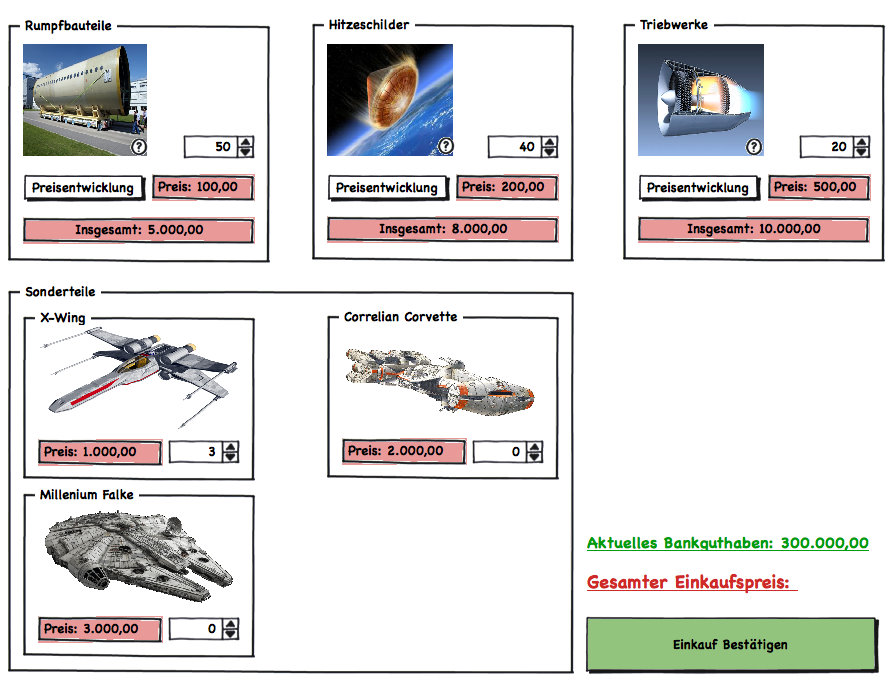
\includegraphics[width=0.9\textwidth]{40_UI/50_Einkauf/Einkauf.jpg}
  }
  \caption{Einkauf}
  \label{img:ui-einkauf}
\end{figure}

\autorende{}